\documentclass[conference]{IEEEtran}
\IEEEoverridecommandlockouts

\usepackage[T1]{fontenc}
\usepackage{cite}
\usepackage{amsmath}
\usepackage{newtxtext,newtxmath}
\usepackage{algorithm}
\usepackage{algpseudocode}
\usepackage{graphicx}
\usepackage{textcomp}
\usepackage{xcolor}
\usepackage{booktabs}
\usepackage{multirow}
\usepackage{array}
\usepackage{pifont}
\usepackage{url}
\usepackage[hidelinks]{hyperref}

\newcommand{\cmark}{\ding{51}}
\newcommand{\xmark}{\ding{55}}
\newcommand{\pmark}{$\circ$}
\newcommand{\code}[1]{\texttt{\small #1}}

\graphicspath{{figures/}}

\begin{document}

\title{Block Vote: A Gasless, Multi-Channel Blockchain E-Voting System with Liveness-Gated Remote Voting and Polling-Station Override}

\author{\IEEEauthorblockN{Deven Wagh}
\IEEEauthorblockA{\textit{Department of Computer Engineering} \\
\textit{Institution Name}\\
City, India}
}

\maketitle

\begin{abstract}
Remote electronic voting promises accessibility but struggles with three recurring problems: voters must be identified without exposing their ballot, coercion in uncontrolled environments, and the cost and complexity that blockchain-based designs push onto voters. We present \emph{Block Vote}, a deployed system that combines (i)~an upgradeable Ethereum smart contract (VotingV3, UUPS proxy, 2-of-3 guardian governance) that records ballots under pseudonymous nullifiers and emits only salted ballot commitments; (ii)~a gasless relay so that voters need no wallet, cryptocurrency, or blockchain knowledge; (iii)~a two-factor voter authentication combining e-mail one-time passwords with cloud face-liveness checks and a 240$^\circ$ device-rotation surround scan on Android; and (iv)~a multi-channel ballot policy in which a voter may cast one remote vote and change it once, while a vote cast at an administrator-activated polling station is final and overrides any remote vote, an operational coercion mitigation inspired by Estonian Internet voting. We describe the architecture, protocols, and implementation (\mbox{$\approx$21,600} lines of Solidity, JavaScript and Kotlin), and evaluate it with 190 automated tests including 30 adversarial scenarios, gas benchmarks cross-validated against 114 live Sepolia transactions, and latency measurements of the production deployment. A first ballot costs 89,946 gas (145,643 gas per voter including registration), i.e.\ $\approx 1.6\times10^{-4}$~ETH at the observed median Sepolia gas price of 1.09~gwei; privacy-preserving commitments and bounded re-voting add 34.7\% over a one-shot baseline. We compare Block Vote with paper-based EVMs, Estonian i-Voting, Helios, Voatz and the Open Vote Network, and discuss the remaining trust in the relay operator.
\end{abstract}

\begin{IEEEkeywords}
blockchain, electronic voting, smart contracts, Ethereum, meta-transactions, liveness detection, coercion resistance, re-voting, UUPS proxy
\end{IEEEkeywords}

% =====================================================================
\section{Introduction}
Elections for universities, cooperatives, professional bodies and local organisations increasingly move online, yet the dominant tools are either conventional web forms, whose integrity rests entirely on the operator, or research systems that ask voters to manage keys and pay transaction fees. Public blockchains~\cite{nakamoto2008,wood2014} offer an append-only, publicly auditable record, but naive designs leak ballots in public events, require every voter to hold a funded wallet, and give no answer to coercion in the home~\cite{park2021}.

Block Vote targets organisational elections with a known electoral roll (an e-mail address per voter) and aims for four practical properties: \emph{eligibility} (only enrolled, physically present humans vote), \emph{uniqueness} (one counted ballot per voter), \emph{public integrity} (tallies are computed by a smart contract and every ballot is an on-chain transaction), and \emph{usability} (no wallet, no fees, a native Android app plus an in-person fallback).

\textbf{Contributions.} This paper makes the following contributions:
\begin{enumerate}
  \item A deployed architecture that couples a gasless relay with an upgradeable voting contract whose vote events carry only salted commitments, never plaintext choices (Section~\ref{sec:arch}).
  \item A \emph{multi-channel ballot policy}: at most two remote ballots (first vote and one change) and a final, overriding polling-station ballot, enforced by an atomic off-chain ledger and reflected on-chain through latest-vote-counts semantics (Section~\ref{sec:channels}).
  \item A liveness pipeline combining cloud face analysis with a 240$^\circ$ device-rotation surround scan that detects additional persons during capture (Section~\ref{sec:liveness}).
  \item An evaluation with 190 automated tests, reproducible gas benchmarks cross-validated on a public testnet, operational cost projections and production latency (Section~\ref{sec:eval}), and a structured comparison with five existing systems (Section~\ref{sec:compare}).
\end{enumerate}

% =====================================================================
\section{Background and Related Work}
\label{sec:related}

\textbf{Supervised electronic voting.} India's standalone Electronic Voting Machines with Voter-Verifiable Paper Audit Trail (VVPAT) provide in-booth secrecy and a paper audit record but require physical presence~\cite{eci_evm}.

\textbf{Internet voting.} Estonia has run binding national Internet voting since 2005 using national ID cards~\cite{madise2006}. Two of its design decisions directly inform ours: voters may \emph{re-vote} online, and a ballot cast in person supersedes an Internet ballot, which weakens the value of coercing a voter at home. Security analyses have nevertheless highlighted its reliance on trusted server-side components~\cite{springall2014}.

\textbf{End-to-end verifiable systems.} Helios~\cite{adida2008} encrypts ballots in the browser, publishes them on a bulletin board and tallies homomorphically, with Benaloh-style cast-as-intended challenges~\cite{benaloh2006}; its author recommends it for low-coercion settings. Receipt-based schemes~\cite{chaum2004} and coercion-resistant protocols based on fake credentials~\cite{juels2005} give stronger guarantees at a considerable usability cost.

\textbf{Blockchain voting.} The Open Vote Network~\cite{mccorry2017} implements self-tallying boardroom voting on Ethereum with maximal ballot secrecy, but every voter needs an Ethereum account and pays gas, and the protocol is limited to small electorates. Numerous proposals use permissioned or public chains for e-voting~\cite{kshetri2018,hjalmarsson2018}. The Voatz mobile application, which combined biometrics with a permissioned blockchain, was shown to have serious vulnerabilities in its client and server design~\cite{specter2020}, and Park~\emph{et al.}~\cite{park2021} argue that blockchains do not by themselves solve the core problems of Internet voting. We take these critiques as design constraints: the blockchain in Block Vote provides public integrity of recorded ballots and tallies, while eligibility, liveness and coercion mitigation are handled explicitly by other mechanisms whose trust assumptions we state.

\textbf{Upgradeability and signatures.} The contract follows the Universal Upgradeable Proxy Standard (UUPS, EIP-1822)~\cite{eip1822}; privileged dashboard actions are authorised with EIP-191 personal signatures~\cite{eip191}. Liveness terminology follows ISO/IEC 30107~\cite{iso30107}, and OTP handling follows NIST SP~800-63B guidance~\cite{nist80063b}.

% =====================================================================
\section{Threat Model and Design Goals}
\label{sec:threat}

\textbf{Actors.} \emph{Voters} (enrolled e-mail addresses); \emph{election administrators} who create elections, candidates and rolls; three \emph{guardians} who approve go-live and contract upgrades; the \emph{relay operator} who runs the application tier and the funded relay wallet; and external \emph{observers} who read the chain.

\textbf{Adversaries.} We consider (A1) ineligible or double voters, (A2) coercers who observe or pressure a voter at home, (A3) a malicious administrator, (A4) a partially compromised backend database, (A5) attacks on contract logic, (A6) network and relay-level attacks, and (A8) collusion among guardians. These map one-to-one onto our adversarial test suite (Table~\ref{tab:attacks}).

\textbf{Trust assumptions.} The relay operator is trusted not to \emph{censor} or \emph{alter} submitted ballots and learns the plaintext candidate at submission time; the identity secret used to derive nullifiers is held only server-side; guardians are honest-majority. We do not claim end-to-end verifiability or cryptographic coercion resistance; Section~\ref{sec:limits} discusses these gaps.

\begin{table}[t]
\caption{Design goals and the mechanisms that realise them}
\label{tab:goals}
\centering
\footnotesize
\begin{tabular}{@{}p{2.05cm}p{5.95cm}@{}}
\toprule
\textbf{Goal} & \textbf{Mechanism in Block Vote} \\
\midrule
Eligibility & Admin-uploaded roll; e-mail OTP (bcrypt, 5\,min, 3 attempts); face liveness; on-chain registration of nullifier \\
Uniqueness & One nullifier per e-mail; latest-vote-counts tally; atomic vote-slot ledger \\
Public integrity & Every ballot is a relay transaction to VotingV3; tallies maintained by contract; audit endpoint verifies tx inclusion \\
Ballot privacy (public) & No PII on chain; \code{VoteCastPrivate} emits $H(e\,\|\,c\,\|\,n\,\|\,s)$ only; receipts omit candidate \\
Coercion mitigation & One remote change of mind; final polling-station override; voting-hours window \\
Usability & No wallet, no fees (gasless relay); native Android app; web ballot at polling stations \\
Governance & 2-of-3 guardian UUPS upgrades; signed guardian actions (5\,min TTL) \\
\bottomrule
\end{tabular}
\end{table}

% =====================================================================
\section{System Architecture}
\label{sec:arch}

Fig.~\ref{fig:arch} shows the three tiers. \emph{Clients} are the Android app (Kotlin, Jetpack Compose, CameraX, ML~Kit), a web ballot that only opens on polling-station computers activated by an administrator, and web dashboards for administrators and guardians. The \emph{application tier} is a Next.js~15 App Router service deployed on Vercel that implements identity, liveness, vote rules, the vote ledger, the gasless relay and authorisation of privileged operations. \emph{External services} are MongoDB Atlas (roll, elections, OTP hashes, relay log), AWS Rekognition (face analysis), Resend (e-mail) and the Ethereum Sepolia test network hosting the VotingV3 proxy.

\begin{figure*}[t]
\centering
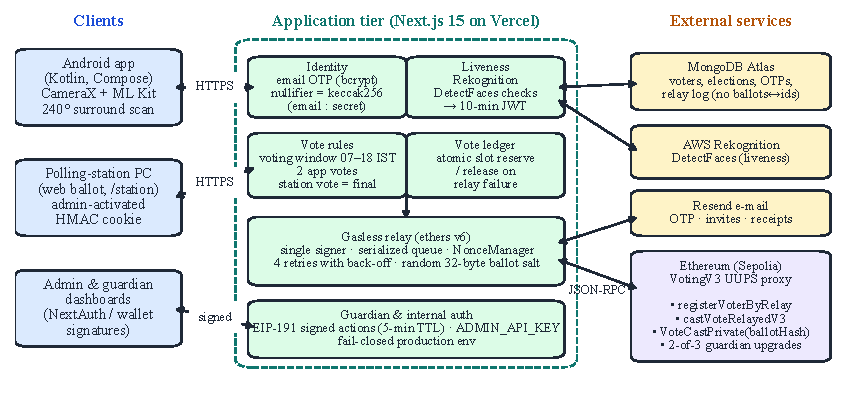
\includegraphics[width=\textwidth]{fig_architecture.pdf}
\caption{Block Vote architecture. Voters never hold keys: all chain writes are relayed by the application tier. Privileged operations require either an administrator session, a guardian wallet signature, or an internal API key.}
\label{fig:arch}
\end{figure*}

\subsection{Smart contract}
VotingV3 (Solidity 0.8.22, OpenZeppelin upgradeable v5) is deployed behind a UUPS proxy. Its state comprises elections (title, description, banner, start/end time, phase $\in\{$Registration, Voting, Completed$\}$), candidates with vote counters, a registration map \code{isRegisteredVoter[e][n]} and, per nullifier $n$ and election $e$, \code{voteChoice[n][e]} (candidate index $+1$) and \code{voteRevisionCount[n][e]}. Election identifiers are \code{keccak256} digests of the title, times, timestamp, sender and index. Mutating functions are restricted to the relay address (\code{onlyRelay}); upgrades follow a propose/approve/execute protocol with \code{APPROVAL\_THRESHOLD}~$=2$ of \code{GUARDIAN\_COUNT}~$=3$.

The core function \code{castVoteRelayedV3}$(e,c,n,s)$ checks registration, the Voting phase and the candidate index; on a first vote it increments the candidate counter; on a re-vote for a different candidate it moves one unit from the previous to the new counter (with an underflow guard). It then stores $c+1$ and emits
\begin{equation}
\text{VoteCastPrivate}\big(e,\; h=\mathrm{keccak256}(e\,\|\,c\,\|\,n\,\|\,s),\; \mathit{isRevote}\big),
\end{equation}
where $s$ is a fresh 32-byte salt chosen by the relay. Unlike the earlier VotingV1, which emitted \code{VoteCast}$(e,c)$ and allowed exactly one ballot, the event never contains the candidate, and tallies always reflect the latest ballot.

\subsection{Voter identity}
A voter's nullifier is $n = \mathrm{keccak256}(\mathit{email}\,\|\,\text{``:''}\,\|\,K_{id})$, where $K_{id}$ is the server identity secret. Observers therefore cannot map on-chain nullifiers to e-mail addresses, while the operator can recompute $n$ to authorise a voter. Biometric session tokens are HS256 JWTs bound to $n$ with a 10-minute lifetime. In production, all secrets and public URLs are read through a fail-closed configuration module that refuses to start when a value is missing.

% =====================================================================
\section{Protocols}
\label{sec:protocols}

\subsection{Liveness and surround scan}
\label{sec:liveness}
On Android the front camera runs CameraX preview and analysis every 90\,ms with ML~Kit face detection. The voter rotates the phone while keeping the face at 10--38\% of the frame height; the rotation-vector sensor accumulates yaw in a locked direction until 240$^\circ$ are covered, and any additional face resets the scan. After 900\,ms of stable single-face framing the app auto-captures a frame and submits it. The server calls Rekognition \code{DetectFaces} and rejects the frame unless exactly one face is present with confidence $\geq 90$, brightness $\geq 30$, no eyeglasses or sunglasses detected with confidence $>80$, and eyes open. Polling stations skip the surround scan because the environment is supervised.

\subsection{Ballot casting}
Fig.~\ref{fig:seq} shows the end-to-end flow. After liveness, the voter requests a 6-digit OTP (\code{crypto.randomInt}, stored as a bcrypt hash, valid 5\,min, at most 3 wrong attempts; 5 requests per minute per IP). \code{verify-otp} validates the OTP and biometric token, checks the election phase and the voting window (default 07:00--18:00 Asia/Kolkata), reserves a vote slot (Algorithm~\ref{alg:slot}), and invokes the relay. The relay serialises transactions through a single queue with an ethers \code{NonceManager}, retries nonce errors up to four times with linear back-off, and records gas usage. On failure the slot is released. The voter receives an e-mail receipt containing the transaction hash but not the candidate; \code{/api/audit/verify} confirms inclusion of a transaction without revealing its content.

\begin{figure*}[t]
\centering
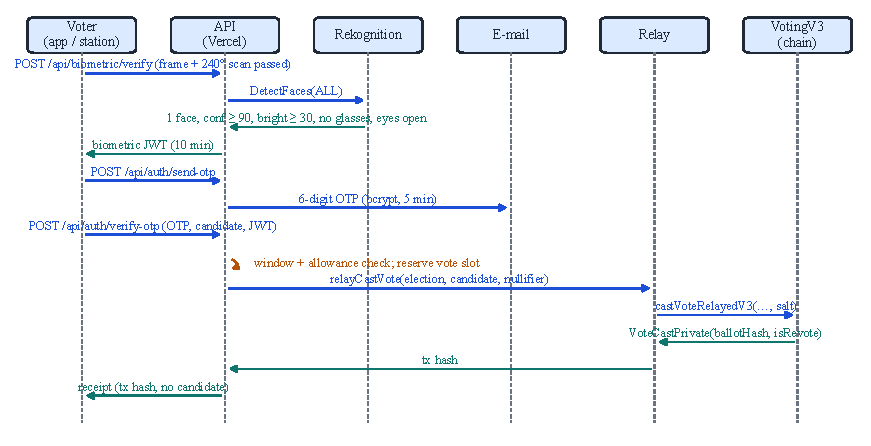
\includegraphics[width=0.94\textwidth]{fig_sequence.pdf}
\caption{Ballot-casting sequence. The candidate reaches the chain only inside contract storage; the public event carries a salted commitment.}
\label{fig:seq}
\end{figure*}

\subsection{Multi-channel ballot policy}
\label{sec:channels}
Remote voting cannot guarantee a private booth. Following the Estonian model, Block Vote lets voters undo a coerced or mistaken remote vote, but bounds the number of remote changes to limit repeated pressure and relay cost. Fig.~\ref{fig:channels} depicts the per-voter state machine: two app ballots are allowed (the latest counts), and a ballot cast at a polling station is final and overrides any app ballot. Because VotingV3 itself permits unlimited re-votes with latest-counts semantics, the policy is enforced in the application tier by an atomic compare-and-increment on the voter document (Algorithm~\ref{alg:slot}); concurrent requests cannot exceed the allowance because the filter and the increment execute as one MongoDB operation.

\begin{figure}[t]
\centering
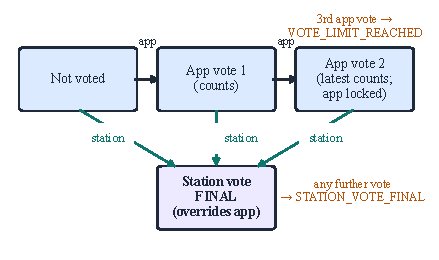
\includegraphics[width=\columnwidth]{fig_channels.pdf}
\caption{Per-voter ballot state machine across the app and polling-station channels.}
\label{fig:channels}
\end{figure}

\begin{algorithm}[t]
\caption{Atomic vote-slot reservation}
\label{alg:slot}
\footnotesize
\begin{algorithmic}[1]
\Require voter id $v$, channel $\in\{\text{app},\text{station}\}$, $M=2$
\State $F \gets \{\_id = v,\ \text{stationVoteFinal} \neq \text{true}\}$
\If{channel $=$ app} \State $F \gets F \wedge \neg(\text{votesCast} \geq M)$ \EndIf
\State $U \gets \{\text{votesCast} \mathrel{+}= 1\}$
\If{channel $=$ station} \State $U \gets U \cup \{\text{stationVoteFinal} \gets \text{true}\}$ \EndIf
\State $b \gets \textsc{FindOneAndUpdate}(F, U, \text{return before})$
\If{$b = \bot$} \Return reject (\textsc{Vote\_Limit\_Reached} or \textsc{Station\_Vote\_Final}) \EndIf
\State $r \gets \textsc{RelayCastVote}(\cdot)$
\If{$r$ failed} \State restore the voter document to $b$ (release slot) \EndIf
\end{algorithmic}
\end{algorithm}

\subsection{Polling-station sessions}
An authenticated administrator activates a computer for one election at \code{/station}; the server sets an \code{httpOnly}, \code{SameSite=Strict} cookie containing a payload (station id, name, election, admin, issue and expiry time, 16\,h lifetime) authenticated with HMAC-SHA256 under a key derived from the station secret. The web ballot at \code{/station/vote} only renders when this cookie verifies, so the web channel cannot be used remotely. The kiosk resets after 2 minutes of inactivity.

\subsection{Governance and privileged operations}
Election go-live requires a guardian approval. Guardians sign an EIP-191 message binding the action, the target election and an issue time; the server recovers the signer with \code{ethers.verifyMessage}, requires the signature to be at most five minutes old and checks the signer against the configured and on-chain guardian lists. The same mechanism protects data wiping and relay-log clearing, so knowledge of a guardian's public address alone confers no authority. Server-to-server synchronisation endpoints require an API key compared in constant time. Contract upgrades require two of three guardians on-chain.

% =====================================================================
\section{Implementation}
\label{sec:impl}

Table~\ref{tab:stack} lists the technology stack and Table~\ref{tab:loc} the code base size (excluding generated code and dependencies). The web tier exposes 56 API route handlers and 11 MongoDB models. The Android app (min SDK 26, target SDK 36) supports \code{blockvote://} deep links and verified HTTPS App Links for invitations, and ships a production flavour restricted to HTTPS via a network security configuration.

\begin{table}[t]
\caption{Technology stack}
\label{tab:stack}
\centering
\footnotesize
\begin{tabular}{@{}ll@{}}
\toprule
\textbf{Layer} & \textbf{Technology (version)} \\
\midrule
Contract & Solidity 0.8.22, OpenZeppelin 5.6 (UUPS) \\
Chain & Hardhat 2.28 (local), Ethereum Sepolia (live) \\
Web / API & Next.js 15.3, React 19.1, Auth.js v5 \\
Chain client & ethers 6.15 (NonceManager relay) \\
Data & MongoDB Atlas, Mongoose 9.2 \\
Biometrics & AWS Rekognition DetectFaces; ML Kit Face 16.1.7 \\
Messaging & Resend 6.17 \\
Android & Kotlin 2.2, Compose, Hilt 2.57, CameraX 1.5 \\
Hosting & Vercel (serverless functions) \\
\bottomrule
\end{tabular}
\end{table}

\begin{table}[t]
\caption{Code base metrics (source lines, September 2026)}
\label{tab:loc}
\centering
\footnotesize
\begin{tabular}{@{}lrr@{}}
\toprule
\textbf{Component} & \textbf{Files} & \textbf{Lines} \\
\midrule
Solidity contracts (V1, V2, V3) & 3 & 959 \\
API route handlers & 56 & 4,735 \\
Web pages and components (JSX) & 44 & 7,699 \\
Server libraries (JS) & 37 & 2,865 \\
Android app (Kotlin) & 42 & 5,351 \\
\midrule
\textbf{Total} & \textbf{182} & \textbf{21,609} \\
\bottomrule
\end{tabular}
\end{table}

% =====================================================================
\section{Evaluation}
\label{sec:eval}

\subsection{Methodology}
Gas was measured with a reproducible script (\code{scripts/benchmark-gas.js}) that deploys the UUPS proxy on the in-process Hardhat network and executes one election with 3 candidates and 50 voters, followed by 25 re-votes to a different candidate and 25 re-votes to the same candidate. To validate these numbers we exported the production relay log, which contains 114 Sepolia transactions (12--21 August 2026) with their receipts' \code{gasUsed} and effective gas price. Production latency was measured from a residential client in India with 20 sequential HTTPS requests per endpoint against the live deployment. Functional correctness was assessed with the automated suites in Table~\ref{tab:tests} and with an end-to-end rule test executed against a running server.

\subsection{Automated tests}
All 190 tests pass (Table~\ref{tab:tests}). The adversarial suite (Table~\ref{tab:attacks}) encodes attacks by voters, coercers, administrators, a compromised backend, contract-level manipulation, relay-level replay and guardian collusion. The production-readiness suite additionally scans the shipped source for development leftovers (test-network keys, hard-coded local URLs, demo toggles), verifies fail-closed configuration and checks guardian signatures against forgery, expiry, replay across elections and non-guardian signers. During this evaluation the suites exposed two real defects that we fixed: 35 contract assertions still expected V1 revert strings, and a production endpoint failed on cold start because a referenced data model was not registered.

\begin{table}[t]
\caption{Automated test suites (all passing)}
\label{tab:tests}
\centering
\footnotesize
\begin{tabular}{@{}lrl@{}}
\toprule
\textbf{Suite} & \textbf{Tests} & \textbf{Scope} \\
\midrule
VotingV3 contract & 75 & lifecycle, re-vote, tallies, UUPS \\
Security attacks (A1--A8) & 30 & adversarial scenarios \\
Production readiness & 26 & env, auth, links, source scan \\
Preflight \& identity & 22 & eligibility cache, commitments \\
Vote rules & 17 & hours, allowance, station token \\
Rate limiting & 13 & sliding window \\
Biometric tokens & 7 & landmarks, JWT \\
\midrule
\textbf{Total} & \textbf{190} & \\
\bottomrule
\end{tabular}
\end{table}

\begin{table}[t]
\caption{Adversarial scenarios covered by the security suite}
\label{tab:attacks}
\centering
\footnotesize
\begin{tabular}{@{}p{1.95cm}p{6.05cm}@{}}
\toprule
\textbf{Adversary} & \textbf{Representative tests} \\
\midrule
A1 Voter & unregistered vote; zero or null-byte nullifier; direct (non-relay) cast or registration; out-of-range candidate; salt replay \\
A2 Coercer & no plaintext candidate in events; legacy event not emitted; coerced vote overwritten by re-vote; commitment brute-force resistance \\
A3 Admin & add candidate during voting; reopen completed election; single-guardian upgrade; direct counter write \\
A4 Backend & nullifier pre-image resistance; salt/identity correlation \\
A5 Contract & immutable config; underflow guard; phase machine; vote conservation \\
A6 Relay & revoked relay privileges; distinct salts yield distinct events \\
A8 Collusion & 2-of-3 guardians can upgrade; one cannot \\
\bottomrule
\end{tabular}
\end{table}

\textbf{End-to-end rule test.} Against a running server with a seeded election, a scripted test confirmed seven properties: first app vote accepted; one change accepted; third app vote rejected (\textsc{Vote\_Limit\_Reached}); station vote accepted and overriding; app vote after station rejected (\textsc{Station\_Vote\_Final}); second station vote rejected; and the on-chain \code{getVoteStatus} matching the off-chain ledger. A station ballot through the browser and an app ballot on a physical Android device (POCO~F7) were also completed with a live face.

\subsection{Gas consumption}
Table~\ref{tab:gas} and Fig.~\ref{fig:gas} report gas per operation. Registration and phase transitions match Sepolia exactly (55,697 vs.\ 55,697 mean; 38,619 vs.\ 38,619), confirming that the benchmark is representative; creation and candidate costs differ only because production strings differ in length. A first ballot costs 89,946 gas; a re-vote costs 77,478 (changed) or 63,974 (same candidate). Relative to the one-shot VotingV1 baseline (66,784 gas), privacy-preserving commitments and re-vote bookkeeping add 23,162 gas (+34.7\%), dominated by one additional zero-to-non-zero storage write for \code{voteChoice}.

\begin{table}[t]
\caption{Gas per operation (Hardhat: 50 voters; Sepolia: live relay log)}
\label{tab:gas}
\centering
\footnotesize
\begin{tabular}{@{}lrrr@{}}
\toprule
\textbf{Operation} & \textbf{V3 Hardhat} & \textbf{V3 Sepolia} & \textbf{V1 baseline} \\
 & mean (n) & mean (n) & mean \\
\midrule
Create election & 238,635 (1) & 223,253 (9) & 238,613 \\
Add candidate & 181,073 (3) & 193,002 (17) & 181,148 \\
Register voter & 55,697 (50) & 55,697 (83) & 55,752 \\
Phase transition & 38,619 (1) & 38,619 (5) & 38,585 \\
First vote & 89,946 (50) & -- & 66,784 \\
Re-vote, changed & 77,478 (25) & -- & n/a \\
Re-vote, same & 63,974 (25) & -- & n/a \\
\bottomrule
\end{tabular}
\end{table}

\begin{figure}[t]
\centering
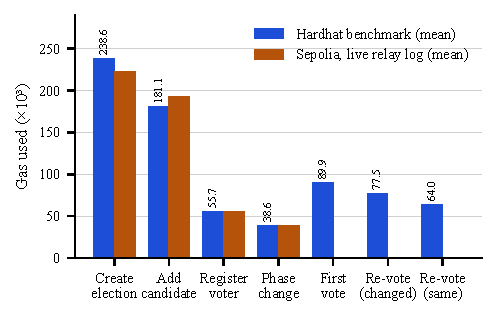
\includegraphics[width=\columnwidth]{fig_gas.pdf}
\caption{Gas per operation: benchmark vs.\ production (Sepolia) relay transactions.}
\label{fig:gas}
\end{figure}

\subsection{Operating cost}
Because voters pay nothing, the operator's marginal cost per voter is registration plus ballots. With one ballot this is $G_1 = 55{,}697 + 89{,}946 = 145{,}643$ gas; the worst case (two app ballots and a station override) is $G_{\max} = 145{,}643 + 2\times 77{,}478 = 300{,}599$ gas. At gas price $p$ (gwei) and $N$ voters, the cost is $C = N\,G\,p\cdot10^{-9}$~ETH. At the observed Sepolia median of 1.09~gwei, one voter costs $1.59\times10^{-4}$~ETH; $10^4$ voters cost 1.46~ETH at 1~gwei and 29.1~ETH at 20~gwei (Fig.~\ref{fig:cost}). The 114 recorded production transactions consumed 0.01224~ETH in total. These figures motivate deployment on low-fee EVM networks (layer-2 rollups or permissioned EVM chains) for large electorates, which requires no contract change.

\begin{figure}[t]
\centering
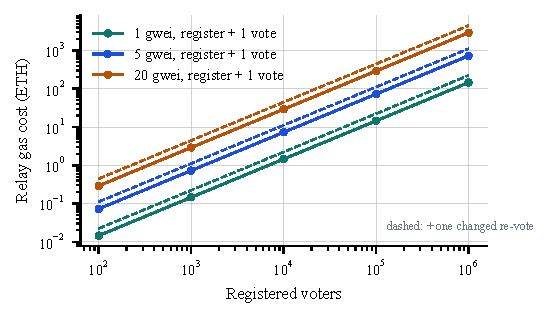
\includegraphics[width=\columnwidth]{fig_cost.pdf}
\caption{Projected relay cost versus electorate size for three gas prices.}
\label{fig:cost}
\end{figure}

\subsection{Throughput}
The relay waits for each receipt inside a single queue per server instance to avoid nonce collisions. Throughput per relay instance is therefore bounded by one confirmed transaction per block, i.e.\ about 300 ballots per hour at Ethereum's 12\,s slot time, independent of gas. A single block with a 30\,M gas limit could hold $\lfloor 30\times10^{6}/89{,}946\rfloor = 333$ first ballots, so batching or pipelined nonces could raise throughput by two orders of magnitude; we list this as future work.

\subsection{Production latency}
Fig.~\ref{fig:latency} shows round-trip latency of the live deployment. Static and light endpoints have a median of 230--260\,ms; endpoints that query MongoDB and the chain have medians of 657--797\,ms. The 95th-percentile outliers (1.7\,s and 5.0\,s) are single samples consistent with serverless cold starts. All 100 requests succeeded.

\begin{figure}[t]
\centering
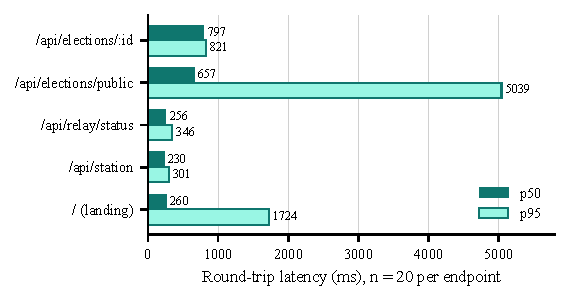
\includegraphics[width=\columnwidth]{fig_latency.pdf}
\caption{Production API latency (p50 and p95, 20 requests per endpoint).}
\label{fig:latency}
\end{figure}

% =====================================================================
\section{Comparison with Existing Systems}
\label{sec:compare}

Table~\ref{tab:compare} compares Block Vote with representative systems using properties reported in the cited literature. Block Vote's distinguishing combination is \emph{remote plus supervised channels with bounded re-voting} (shared only with Estonian i-Voting), a \emph{public ledger without voter wallets or fees} (unlike the Open Vote Network), and \emph{liveness-gated remote access}. Its main weakness relative to Helios and the Open Vote Network is ballot secrecy against the operator: the relay sees the plaintext choice and \code{voteChoice} is readable by anyone who can compute nullifiers.

\begin{table*}[t]
\caption{Qualitative comparison with existing voting systems (\cmark~provided, \pmark~partial or conditional, \xmark~not provided)}
\label{tab:compare}
\centering
\footnotesize
\resizebox{\textwidth}{!}{%
\begin{tabular}{@{}lcccccc@{}}
\toprule
\textbf{Property} & \textbf{EVM + VVPAT}~\cite{eci_evm} & \textbf{Estonia i-Voting}~\cite{madise2006,springall2014} & \textbf{Helios}~\cite{adida2008} & \textbf{Voatz}~\cite{specter2020} & \textbf{Open Vote Net.}~\cite{mccorry2017} & \textbf{Block Vote} \\
\midrule
Remote voting & \xmark & \cmark & \cmark & \cmark & \cmark & \cmark \\
Supervised in-person channel & \cmark & \cmark & \xmark & \xmark & \xmark & \cmark \\
Re-voting / in-person override & \xmark & \cmark & \pmark & \xmark & \xmark & \cmark~(bounded) \\
Public tamper-evident record & \xmark & \xmark & \cmark~(bulletin board) & \pmark~(permissioned) & \cmark & \cmark~(Ethereum) \\
Universally verifiable tally & \pmark~(paper audit) & \xmark & \cmark & \xmark & \cmark & \pmark~(on-chain counters) \\
Ballot secrecy vs.\ public & \cmark & \cmark & \cmark & \pmark & \cmark & \cmark~(commitments) \\
Ballot secrecy vs.\ operator & \cmark & \pmark~(key holders) & \pmark~(trustees) & \xmark & \cmark & \xmark~(relay sees choice) \\
Automated liveness / biometrics & \xmark~(manual ID) & \xmark & \xmark & \cmark & \xmark & \cmark~(liveness only) \\
No voter wallet or fees & \cmark & \cmark & \cmark & \cmark & \xmark & \cmark \\
Contract/system upgrade governance & n/a & n/a & n/a & n/a & \xmark & \cmark~(2-of-3 UUPS) \\
Demonstrated scale & national & national & organisational & pilots & boardroom & prototype \\
\bottomrule
\end{tabular}}
\end{table*}

Quantitatively, the only directly comparable measurement we report is against our own one-shot baseline (Table~\ref{tab:gas}): bounded re-voting and salted commitments cost +34.7\% gas per first ballot. Unlike the Open Vote Network, whose voters each submit transactions, all Block Vote transactions are issued by one relay, so per-voter on-chain cost is independent of client capabilities and hidden from the voter.

% =====================================================================
\section{Security Discussion and Limitations}
\label{sec:limits}

\textbf{Relay trust.} A single relay key submits all ballots; the operator could censor or reorder ballots and sees each choice. Mitigations include publishing the relay log and on-chain counts, and future use of client-side encryption with threshold decryption, or client-signed meta-transactions (e.g.\ EIP-2771) so that the contract verifies voter intent.

\textbf{Pseudonymity, not anonymity.} \code{voteChoice} is public per nullifier and nullifiers are emitted at registration. Secrecy against the public rests on $K_{id}$; an operator or a leaked $K_{id}$ plus the roll links ballots to voters. Replacing stored choices with homomorphic or mix-net tallying would remove this linkage at additional cost.

\textbf{Coercion.} Bounded re-voting and the polling-station override are operational, not cryptographic, defences~\cite{juels2005}; a coercer who controls a voter until polls close is not defeated.

\textbf{Liveness versus identity.} The server checks liveness and image quality but does not match the face against an enrolled reference, so an enrolled voter could let another live person vote after completing OTP. Enrolment-time face matching or ISO/IEC 30107-3 evaluated presentation-attack detection~\cite{iso30107} would strengthen this.

\textbf{Operational gaps.} Go-live approval requires one guardian (contract upgrades require two) and upgrades have no timelock; request rate limiting is kept in per-instance memory, which is weak on serverless platforms; relay throughput is limited per instance; and the Android client has minimal automated tests. The production gas-analytics endpoint is publicly readable, which exposes operational metadata.

% =====================================================================
\section{Conclusion and Future Work}
Block Vote shows that a public-chain voting back end can be made invisible to voters: no wallets, no fees, a native mobile app, and a supervised fallback, while every ballot and tally update remains an auditable on-chain transaction. The multi-channel policy (two remote ballots, final polling-station override) offers a practical, low-cost coercion mitigation, and our measurements show a per-voter cost of 145,643 gas with production API medians below 0.8\,s. Future work targets (i)~client-side ballot encryption with threshold tallying to remove operator visibility, (ii)~pipelined or batched relaying and layer-2 deployment for throughput and cost, (iii)~enrolment-time face matching, and (iv)~a shared rate-limit store and timelocked upgrades.

\section*{Artifact Availability}
The repository contains the gas benchmark (\code{Voting/scripts/benchmark-gas.js}), all test suites, and the measurement data and figure scripts used in this paper (\code{docs/paper/}).

\begin{thebibliography}{00}
\bibitem{nakamoto2008} S. Nakamoto, ``Bitcoin: A peer-to-peer electronic cash system,'' 2008. [Online]. Available: \url{https://bitcoin.org/bitcoin.pdf}
\bibitem{wood2014} G. Wood, ``Ethereum: A secure decentralised generalised transaction ledger,'' Ethereum Yellow Paper, 2014.
\bibitem{park2021} S. Park, M. Specter, N. Narula, and R. L. Rivest, ``Going from bad to worse: From Internet voting to blockchain voting,'' \emph{J. Cybersecurity}, vol.~7, no.~1, 2021.
\bibitem{eci_evm} Election Commission of India, ``Status paper on Electronic Voting Machine (EVM),'' New Delhi, India.
\bibitem{madise2006} \"U. Madise and T. Martens, ``E-voting in Estonia 2005: The first practice of country-wide binding Internet voting in the world,'' in \emph{Proc. Electronic Voting (EVOTE)}, GI LNI P-86, 2006, pp.~15--26.
\bibitem{springall2014} D. Springall \emph{et al.}, ``Security analysis of the Estonian Internet voting system,'' in \emph{Proc. ACM CCS}, 2014, pp.~703--715.
\bibitem{adida2008} B. Adida, ``Helios: Web-based open-audit voting,'' in \emph{Proc. 17th USENIX Security Symp.}, 2008, pp.~335--348.
\bibitem{benaloh2006} J. Benaloh, ``Simple verifiable elections,'' in \emph{Proc. USENIX/ACCURATE Electronic Voting Technology Workshop (EVT)}, 2006.
\bibitem{chaum2004} D. Chaum, ``Secret-ballot receipts: True voter-verifiable elections,'' \emph{IEEE Security \& Privacy}, vol.~2, no.~1, pp.~38--47, 2004.
\bibitem{juels2005} A. Juels, D. Catalano, and M. Jakobsson, ``Coercion-resistant electronic elections,'' in \emph{Proc. ACM Workshop on Privacy in the Electronic Society (WPES)}, 2005, pp.~61--70.
\bibitem{mccorry2017} P. McCorry, S. F. Shahandashti, and F. Hao, ``A smart contract for boardroom voting with maximum voter privacy,'' in \emph{Financial Cryptography and Data Security (FC)}, LNCS 10322, 2017, pp.~357--375.
\bibitem{kshetri2018} N. Kshetri and J. Voas, ``Blockchain-enabled e-voting,'' \emph{IEEE Software}, vol.~35, no.~4, pp.~95--99, 2018.
\bibitem{hjalmarsson2018} F. P. Hj\'{a}lmarsson, G. K. Hrei\dh arsson, M. Hamdaqa, and G. Hj\'{a}lmt\'{y}sson, ``Blockchain-based e-voting system,'' in \emph{Proc. IEEE 11th Int. Conf. Cloud Computing (CLOUD)}, 2018, pp.~983--986.
\bibitem{specter2020} M. A. Specter, J. Koppel, and D. Weitzner, ``The ballot is busted before the blockchain: A security analysis of Voatz, the first Internet voting application used in U.S. federal elections,'' in \emph{Proc. 29th USENIX Security Symp.}, 2020, pp.~1535--1553.
\bibitem{eip1822} G. Barros and P. Gallagher, ``EIP-1822: Universal Upgradeable Proxy Standard (UUPS),'' Ethereum Improvement Proposals, 2019.
\bibitem{eip191} M. Swende and N. Johnson, ``EIP-191: Signed data standard,'' Ethereum Improvement Proposals, 2016.
\bibitem{iso30107} ISO/IEC 30107-3:2017, \emph{Information technology---Biometric presentation attack detection---Part 3: Testing and reporting}.
\bibitem{nist80063b} P. A. Grassi \emph{et al.}, ``Digital identity guidelines: Authentication and lifecycle management,'' NIST SP 800-63B, 2017.
\end{thebibliography}

\end{document}
